% Options for packages loaded elsewhere
\PassOptionsToPackage{unicode}{hyperref}
\PassOptionsToPackage{hyphens}{url}
\PassOptionsToPackage{dvipsnames,svgnames,x11names}{xcolor}
%
\documentclass[
  letterpaper,
  DIV=11,
  numbers=noendperiod]{scrartcl}

\usepackage{amsmath,amssymb}
\usepackage{iftex}
\ifPDFTeX
  \usepackage[T1]{fontenc}
  \usepackage[utf8]{inputenc}
  \usepackage{textcomp} % provide euro and other symbols
\else % if luatex or xetex
  \usepackage{unicode-math}
  \defaultfontfeatures{Scale=MatchLowercase}
  \defaultfontfeatures[\rmfamily]{Ligatures=TeX,Scale=1}
\fi
\usepackage{lmodern}
\ifPDFTeX\else  
    % xetex/luatex font selection
\fi
% Use upquote if available, for straight quotes in verbatim environments
\IfFileExists{upquote.sty}{\usepackage{upquote}}{}
\IfFileExists{microtype.sty}{% use microtype if available
  \usepackage[]{microtype}
  \UseMicrotypeSet[protrusion]{basicmath} % disable protrusion for tt fonts
}{}
\makeatletter
\@ifundefined{KOMAClassName}{% if non-KOMA class
  \IfFileExists{parskip.sty}{%
    \usepackage{parskip}
  }{% else
    \setlength{\parindent}{0pt}
    \setlength{\parskip}{6pt plus 2pt minus 1pt}}
}{% if KOMA class
  \KOMAoptions{parskip=half}}
\makeatother
\usepackage{xcolor}
\setlength{\emergencystretch}{3em} % prevent overfull lines
\setcounter{secnumdepth}{-\maxdimen} % remove section numbering
% Make \paragraph and \subparagraph free-standing
\ifx\paragraph\undefined\else
  \let\oldparagraph\paragraph
  \renewcommand{\paragraph}[1]{\oldparagraph{#1}\mbox{}}
\fi
\ifx\subparagraph\undefined\else
  \let\oldsubparagraph\subparagraph
  \renewcommand{\subparagraph}[1]{\oldsubparagraph{#1}\mbox{}}
\fi

\usepackage{color}
\usepackage{fancyvrb}
\newcommand{\VerbBar}{|}
\newcommand{\VERB}{\Verb[commandchars=\\\{\}]}
\DefineVerbatimEnvironment{Highlighting}{Verbatim}{commandchars=\\\{\}}
% Add ',fontsize=\small' for more characters per line
\usepackage{framed}
\definecolor{shadecolor}{RGB}{241,243,245}
\newenvironment{Shaded}{\begin{snugshade}}{\end{snugshade}}
\newcommand{\AlertTok}[1]{\textcolor[rgb]{0.68,0.00,0.00}{#1}}
\newcommand{\AnnotationTok}[1]{\textcolor[rgb]{0.37,0.37,0.37}{#1}}
\newcommand{\AttributeTok}[1]{\textcolor[rgb]{0.40,0.45,0.13}{#1}}
\newcommand{\BaseNTok}[1]{\textcolor[rgb]{0.68,0.00,0.00}{#1}}
\newcommand{\BuiltInTok}[1]{\textcolor[rgb]{0.00,0.23,0.31}{#1}}
\newcommand{\CharTok}[1]{\textcolor[rgb]{0.13,0.47,0.30}{#1}}
\newcommand{\CommentTok}[1]{\textcolor[rgb]{0.37,0.37,0.37}{#1}}
\newcommand{\CommentVarTok}[1]{\textcolor[rgb]{0.37,0.37,0.37}{\textit{#1}}}
\newcommand{\ConstantTok}[1]{\textcolor[rgb]{0.56,0.35,0.01}{#1}}
\newcommand{\ControlFlowTok}[1]{\textcolor[rgb]{0.00,0.23,0.31}{#1}}
\newcommand{\DataTypeTok}[1]{\textcolor[rgb]{0.68,0.00,0.00}{#1}}
\newcommand{\DecValTok}[1]{\textcolor[rgb]{0.68,0.00,0.00}{#1}}
\newcommand{\DocumentationTok}[1]{\textcolor[rgb]{0.37,0.37,0.37}{\textit{#1}}}
\newcommand{\ErrorTok}[1]{\textcolor[rgb]{0.68,0.00,0.00}{#1}}
\newcommand{\ExtensionTok}[1]{\textcolor[rgb]{0.00,0.23,0.31}{#1}}
\newcommand{\FloatTok}[1]{\textcolor[rgb]{0.68,0.00,0.00}{#1}}
\newcommand{\FunctionTok}[1]{\textcolor[rgb]{0.28,0.35,0.67}{#1}}
\newcommand{\ImportTok}[1]{\textcolor[rgb]{0.00,0.46,0.62}{#1}}
\newcommand{\InformationTok}[1]{\textcolor[rgb]{0.37,0.37,0.37}{#1}}
\newcommand{\KeywordTok}[1]{\textcolor[rgb]{0.00,0.23,0.31}{#1}}
\newcommand{\NormalTok}[1]{\textcolor[rgb]{0.00,0.23,0.31}{#1}}
\newcommand{\OperatorTok}[1]{\textcolor[rgb]{0.37,0.37,0.37}{#1}}
\newcommand{\OtherTok}[1]{\textcolor[rgb]{0.00,0.23,0.31}{#1}}
\newcommand{\PreprocessorTok}[1]{\textcolor[rgb]{0.68,0.00,0.00}{#1}}
\newcommand{\RegionMarkerTok}[1]{\textcolor[rgb]{0.00,0.23,0.31}{#1}}
\newcommand{\SpecialCharTok}[1]{\textcolor[rgb]{0.37,0.37,0.37}{#1}}
\newcommand{\SpecialStringTok}[1]{\textcolor[rgb]{0.13,0.47,0.30}{#1}}
\newcommand{\StringTok}[1]{\textcolor[rgb]{0.13,0.47,0.30}{#1}}
\newcommand{\VariableTok}[1]{\textcolor[rgb]{0.07,0.07,0.07}{#1}}
\newcommand{\VerbatimStringTok}[1]{\textcolor[rgb]{0.13,0.47,0.30}{#1}}
\newcommand{\WarningTok}[1]{\textcolor[rgb]{0.37,0.37,0.37}{\textit{#1}}}

\providecommand{\tightlist}{%
  \setlength{\itemsep}{0pt}\setlength{\parskip}{0pt}}\usepackage{longtable,booktabs,array}
\usepackage{calc} % for calculating minipage widths
% Correct order of tables after \paragraph or \subparagraph
\usepackage{etoolbox}
\makeatletter
\patchcmd\longtable{\par}{\if@noskipsec\mbox{}\fi\par}{}{}
\makeatother
% Allow footnotes in longtable head/foot
\IfFileExists{footnotehyper.sty}{\usepackage{footnotehyper}}{\usepackage{footnote}}
\makesavenoteenv{longtable}
\usepackage{graphicx}
\makeatletter
\def\maxwidth{\ifdim\Gin@nat@width>\linewidth\linewidth\else\Gin@nat@width\fi}
\def\maxheight{\ifdim\Gin@nat@height>\textheight\textheight\else\Gin@nat@height\fi}
\makeatother
% Scale images if necessary, so that they will not overflow the page
% margins by default, and it is still possible to overwrite the defaults
% using explicit options in \includegraphics[width, height, ...]{}
\setkeys{Gin}{width=\maxwidth,height=\maxheight,keepaspectratio}
% Set default figure placement to htbp
\makeatletter
\def\fps@figure{htbp}
\makeatother

\KOMAoption{captions}{tableheading}
\makeatletter
\@ifpackageloaded{tcolorbox}{}{\usepackage[skins,breakable]{tcolorbox}}
\@ifpackageloaded{fontawesome5}{}{\usepackage{fontawesome5}}
\definecolor{quarto-callout-color}{HTML}{909090}
\definecolor{quarto-callout-note-color}{HTML}{0758E5}
\definecolor{quarto-callout-important-color}{HTML}{CC1914}
\definecolor{quarto-callout-warning-color}{HTML}{EB9113}
\definecolor{quarto-callout-tip-color}{HTML}{00A047}
\definecolor{quarto-callout-caution-color}{HTML}{FC5300}
\definecolor{quarto-callout-color-frame}{HTML}{acacac}
\definecolor{quarto-callout-note-color-frame}{HTML}{4582ec}
\definecolor{quarto-callout-important-color-frame}{HTML}{d9534f}
\definecolor{quarto-callout-warning-color-frame}{HTML}{f0ad4e}
\definecolor{quarto-callout-tip-color-frame}{HTML}{02b875}
\definecolor{quarto-callout-caution-color-frame}{HTML}{fd7e14}
\makeatother
\makeatletter
\makeatother
\makeatletter
\makeatother
\makeatletter
\@ifpackageloaded{caption}{}{\usepackage{caption}}
\AtBeginDocument{%
\ifdefined\contentsname
  \renewcommand*\contentsname{Table of contents}
\else
  \newcommand\contentsname{Table of contents}
\fi
\ifdefined\listfigurename
  \renewcommand*\listfigurename{List of Figures}
\else
  \newcommand\listfigurename{List of Figures}
\fi
\ifdefined\listtablename
  \renewcommand*\listtablename{List of Tables}
\else
  \newcommand\listtablename{List of Tables}
\fi
\ifdefined\figurename
  \renewcommand*\figurename{Figure}
\else
  \newcommand\figurename{Figure}
\fi
\ifdefined\tablename
  \renewcommand*\tablename{Table}
\else
  \newcommand\tablename{Table}
\fi
}
\@ifpackageloaded{float}{}{\usepackage{float}}
\floatstyle{ruled}
\@ifundefined{c@chapter}{\newfloat{codelisting}{h}{lop}}{\newfloat{codelisting}{h}{lop}[chapter]}
\floatname{codelisting}{Listing}
\newcommand*\listoflistings{\listof{codelisting}{List of Listings}}
\makeatother
\makeatletter
\@ifpackageloaded{caption}{}{\usepackage{caption}}
\@ifpackageloaded{subcaption}{}{\usepackage{subcaption}}
\makeatother
\makeatletter
\@ifpackageloaded{tcolorbox}{}{\usepackage[skins,breakable]{tcolorbox}}
\makeatother
\makeatletter
\@ifundefined{shadecolor}{\definecolor{shadecolor}{rgb}{.97, .97, .97}}
\makeatother
\makeatletter
\makeatother
\makeatletter
\makeatother
\ifLuaTeX
  \usepackage{selnolig}  % disable illegal ligatures
\fi
\IfFileExists{bookmark.sty}{\usepackage{bookmark}}{\usepackage{hyperref}}
\IfFileExists{xurl.sty}{\usepackage{xurl}}{} % add URL line breaks if available
\urlstyle{same} % disable monospaced font for URLs
\hypersetup{
  pdftitle={Homework 2},
  pdfauthor={Matt Viana},
  colorlinks=true,
  linkcolor={blue},
  filecolor={Maroon},
  citecolor={Blue},
  urlcolor={Blue},
  pdfcreator={LaTeX via pandoc}}

\title{Homework 2}
\author{{Matt Viana}}
\date{}

\begin{document}
\maketitle
\ifdefined\Shaded\renewenvironment{Shaded}{\begin{tcolorbox}[sharp corners, interior hidden, frame hidden, breakable, boxrule=0pt, borderline west={3pt}{0pt}{shadecolor}, enhanced]}{\end{tcolorbox}}\fi

\renewcommand*\contentsname{Table of contents}
{
\hypersetup{linkcolor=}
\setcounter{tocdepth}{3}
\tableofcontents
}
\href{https://github.com/STAT380/hw2.git}{Link to the Github repository}

\begin{center}\rule{0.5\linewidth}{0.5pt}\end{center}

\begin{tcolorbox}[enhanced jigsaw, opacityback=0, colback=white, rightrule=.15mm, colframe=quarto-callout-important-color-frame, opacitybacktitle=0.6, title=\textcolor{quarto-callout-important-color}{\faExclamation}\hspace{0.5em}{Due: Feb 9, 2024 @ 11:59pm}, breakable, bottomtitle=1mm, arc=.35mm, titlerule=0mm, toptitle=1mm, leftrule=.75mm, left=2mm, bottomrule=.15mm, toprule=.15mm, coltitle=black, colbacktitle=quarto-callout-important-color!10!white]

Please read the instructions carefully before submitting your
assignment.

\begin{enumerate}
\def\labelenumi{\arabic{enumi}.}
\tightlist
\item
  This assignment requires you to only upload a \texttt{PDF} file on
  Canvas
\item
  Don't collapse any code cells before submitting.
\item
  Remember to make sure all your code output is rendered properly before
  uploading your submission.
\end{enumerate}

⚠️ Please add your name to the author information in the frontmatter
before submitting your assignment ⚠️

\end{tcolorbox}

For this assignment, we will be using the
\href{http://archive.ics.uci.edu/ml/datasets/Abalone}{Abalone dataset}
from the UCI Machine Learning Repository. The dataset consists of
physical measurements of abalone (a type of marine snail) and includes
information on the age, sex, and size of the abalone.

We will be using the following libraries:

\begin{Shaded}
\begin{Highlighting}[]
\FunctionTok{library}\NormalTok{(readr)}
\FunctionTok{library}\NormalTok{(tidyr)}
\FunctionTok{library}\NormalTok{(ggplot2)}
\FunctionTok{library}\NormalTok{(dplyr)}
\end{Highlighting}
\end{Shaded}

\begin{verbatim}

Attaching package: 'dplyr'
\end{verbatim}

\begin{verbatim}
The following objects are masked from 'package:stats':

    filter, lag
\end{verbatim}

\begin{verbatim}
The following objects are masked from 'package:base':

    intersect, setdiff, setequal, union
\end{verbatim}

\begin{Shaded}
\begin{Highlighting}[]
\FunctionTok{library}\NormalTok{(purrr)}
\FunctionTok{library}\NormalTok{(cowplot)}
\end{Highlighting}
\end{Shaded}

\hypertarget{section}{%
\subsection{\texorpdfstring{}{    }}\label{section}}

\hypertarget{question-1}{%
\subsection{Question 1}\label{question-1}}

\begin{tcolorbox}[enhanced jigsaw, opacityback=0, colback=white, rightrule=.15mm, colframe=quarto-callout-tip-color-frame, opacitybacktitle=0.6, title=\textcolor{quarto-callout-tip-color}{\faLightbulb}\hspace{0.5em}{30 points}, breakable, bottomtitle=1mm, arc=.35mm, titlerule=0mm, toptitle=1mm, leftrule=.75mm, left=2mm, bottomrule=.15mm, toprule=.15mm, coltitle=black, colbacktitle=quarto-callout-tip-color!10!white]

EDA using \texttt{readr}, \texttt{tidyr} and \texttt{ggplot2}

\end{tcolorbox}

1.1 (5 points)

Load the ``Abalone'' dataset as a tibble called \texttt{abalone} using
the URL provided below. The \texttt{abalone\_col\_names} variable
contains a vector of the column names for this dataset (to be consistent
with the R naming pattern). Make sure you read the dataset with the
provided column names.

\begin{Shaded}
\begin{Highlighting}[]
\FunctionTok{library}\NormalTok{(readr)}
\NormalTok{url }\OtherTok{\textless{}{-}} \StringTok{"http://archive.ics.uci.edu/ml/machine{-}learning{-}databases/abalone/abalone.data"}

\NormalTok{abalone\_col\_names }\OtherTok{\textless{}{-}} \FunctionTok{c}\NormalTok{(}
  \StringTok{"sex"}\NormalTok{, }
  \StringTok{"length"}\NormalTok{, }
  \StringTok{"diameter"}\NormalTok{, }
  \StringTok{"height"}\NormalTok{, }
  \StringTok{"whole\_weight"}\NormalTok{, }
  \StringTok{"shucked\_weight"}\NormalTok{, }
  \StringTok{"viscera\_weight"}\NormalTok{, }
  \StringTok{"shell\_weight"}\NormalTok{, }
  \StringTok{"rings"}
\NormalTok{)}

\NormalTok{abalone }\OtherTok{\textless{}{-}} \FunctionTok{read\_csv}\NormalTok{(url, }\AttributeTok{col\_names =}\NormalTok{ abalone\_col\_names, }\AttributeTok{show\_col\_types =} \ConstantTok{FALSE}\NormalTok{)}
\end{Highlighting}
\end{Shaded}

\begin{center}\rule{0.5\linewidth}{0.5pt}\end{center}

1.2 (5 points)

Remove missing values and \texttt{NA}s from the dataset and store the
cleaned data in a tibble called \texttt{df}. How many rows were dropped?

\begin{Shaded}
\begin{Highlighting}[]
\NormalTok{df }\OtherTok{\textless{}{-}} \FunctionTok{na.omit}\NormalTok{(abalone)}
\end{Highlighting}
\end{Shaded}

\begin{center}\rule{0.5\linewidth}{0.5pt}\end{center}

\hypertarget{points-3}{%
\subparagraph{1.3 (5 points)}\label{points-3}}

Plot histograms of all the quantitative variables in a \textbf{single
plot} \footnote{You can use the \texttt{facet\_wrap()} function for
  this. Have a look at its documentation using the help console in R}

\begin{Shaded}
\begin{Highlighting}[]
\NormalTok{dff }\OtherTok{\textless{}{-}} \FunctionTok{as.double}\NormalTok{(}\FunctionTok{unlist}\NormalTok{(df))}
\end{Highlighting}
\end{Shaded}

\begin{verbatim}
Warning: NAs introduced by coercion
\end{verbatim}

\begin{Shaded}
\begin{Highlighting}[]
\FunctionTok{hist}\NormalTok{(dff, }\AttributeTok{main =} \StringTok{"Histogram of abalone"}\NormalTok{)}
\end{Highlighting}
\end{Shaded}

\begin{figure}[H]

{\centering 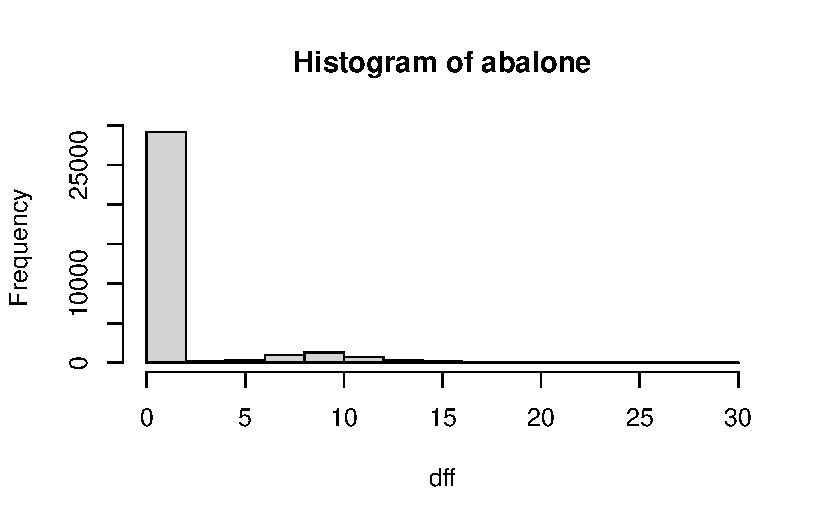
\includegraphics{hw2_files/figure-pdf/unnamed-chunk-4-1.pdf}

}

\end{figure}

\begin{center}\rule{0.5\linewidth}{0.5pt}\end{center}

\hypertarget{points-4}{%
\subparagraph{1.4 (5 points)}\label{points-4}}

Create a boxplot of \texttt{length} for each \texttt{sex} and create a
violin-plot of of \texttt{diameter} for each \texttt{sex}. Are there any
notable differences in the physical appearences of abalones based on
your analysis here?

\begin{Shaded}
\begin{Highlighting}[]
\FunctionTok{boxplot}\NormalTok{(length }\SpecialCharTok{\textasciitilde{}}\NormalTok{ sex, }\AttributeTok{data =}\NormalTok{ abalone, }
        \AttributeTok{main =} \StringTok{"Boxplot of Length by Sex"}\NormalTok{,}
        \AttributeTok{xlab =} \StringTok{"Sex"}\NormalTok{, }\AttributeTok{ylab =} \StringTok{"Length"}\NormalTok{)}
\end{Highlighting}
\end{Shaded}

\begin{figure}[H]

{\centering 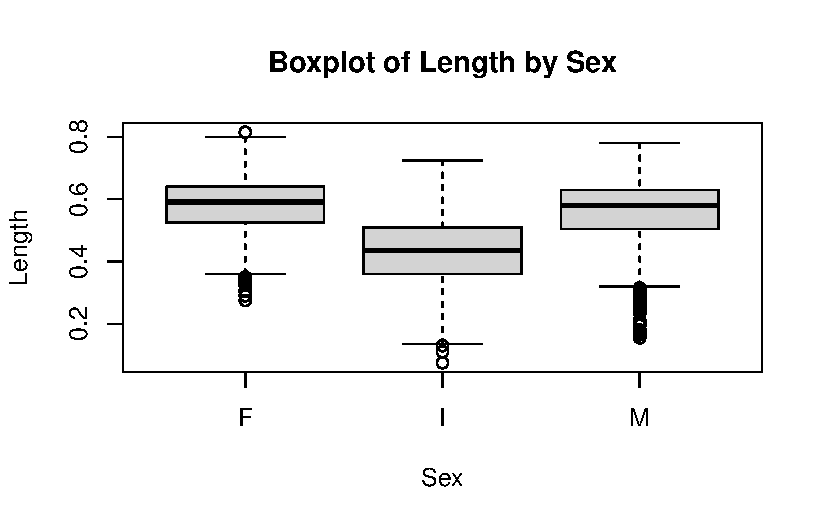
\includegraphics{hw2_files/figure-pdf/unnamed-chunk-5-1.pdf}

}

\end{figure}

\begin{Shaded}
\begin{Highlighting}[]
\FunctionTok{ggplot}\NormalTok{(abalone, }\FunctionTok{aes}\NormalTok{(}\AttributeTok{x =}\NormalTok{ sex, }\AttributeTok{y =}\NormalTok{ diameter, }\AttributeTok{fill =}\NormalTok{ sex)) }\SpecialCharTok{+}
  \FunctionTok{geom\_violin}\NormalTok{() }\SpecialCharTok{+}
  \FunctionTok{labs}\NormalTok{(}\AttributeTok{title =} \StringTok{"Violin Plot of Diameter by Sex"}\NormalTok{, }\AttributeTok{x =} \StringTok{"Sex"}\NormalTok{, }\AttributeTok{y =} \StringTok{"Diameter"}\NormalTok{)}
\end{Highlighting}
\end{Shaded}

\begin{figure}[H]

{\centering 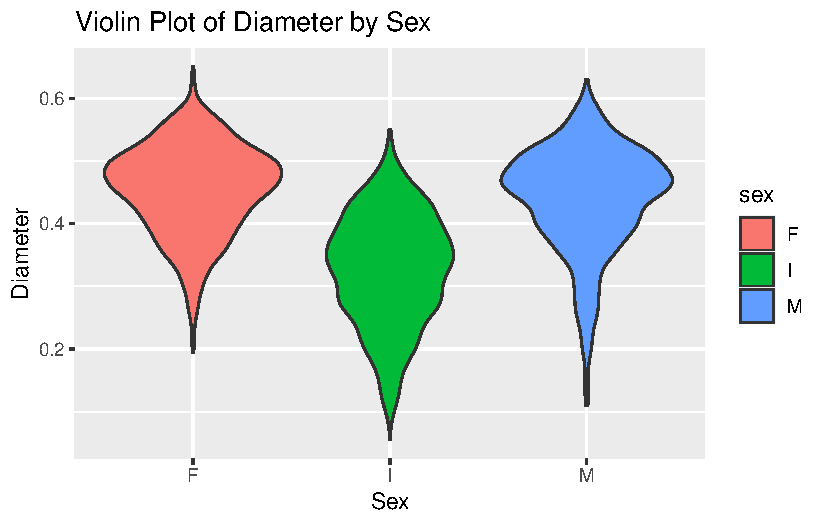
\includegraphics{hw2_files/figure-pdf/unnamed-chunk-6-1.pdf}

}

\end{figure}

The Violin plot is more organic. It doesn't have steps like the boxplot
does. You can look at each area instead of the whole..

\begin{center}\rule{0.5\linewidth}{0.5pt}\end{center}

1.5 (5 points)

Create a scatter plot of \texttt{length} and \texttt{diameter}, and
modify the shape and color of the points based on the \texttt{sex}
variable. Change the size of each point based on the
\texttt{shell\_wight} value for each observation. Are there any notable
anomalies in the dataset?

\begin{Shaded}
\begin{Highlighting}[]
\FunctionTok{ggplot}\NormalTok{(abalone, }\FunctionTok{aes}\NormalTok{(}\AttributeTok{x =}\NormalTok{ length, }\AttributeTok{y =}\NormalTok{ diameter, }\AttributeTok{color =}\NormalTok{ sex, }\AttributeTok{shape =}\NormalTok{ sex, }\AttributeTok{size =}\NormalTok{ shell\_weight)) }\SpecialCharTok{+}
  \FunctionTok{geom\_point}\NormalTok{() }\SpecialCharTok{+}
  \FunctionTok{labs}\NormalTok{(}\AttributeTok{title =} \StringTok{"Scatter Plot of Length vs. Diameter"}\NormalTok{,}
       \AttributeTok{x =} \StringTok{"Length"}\NormalTok{, }\AttributeTok{y =} \StringTok{"Diameter"}\NormalTok{) }\SpecialCharTok{+}
  \FunctionTok{scale\_color\_manual}\NormalTok{(}\AttributeTok{values =} \FunctionTok{c}\NormalTok{(}\StringTok{"blue"}\NormalTok{, }\StringTok{"red"}\NormalTok{, }\StringTok{"green"}\NormalTok{)) }\SpecialCharTok{+}
  \FunctionTok{scale\_shape\_manual}\NormalTok{(}\AttributeTok{values =} \FunctionTok{c}\NormalTok{(}\DecValTok{19}\NormalTok{, }\DecValTok{17}\NormalTok{, }\DecValTok{15}\NormalTok{)) }\SpecialCharTok{+}
  \FunctionTok{theme\_minimal}\NormalTok{()}
\end{Highlighting}
\end{Shaded}

\begin{figure}[H]

{\centering 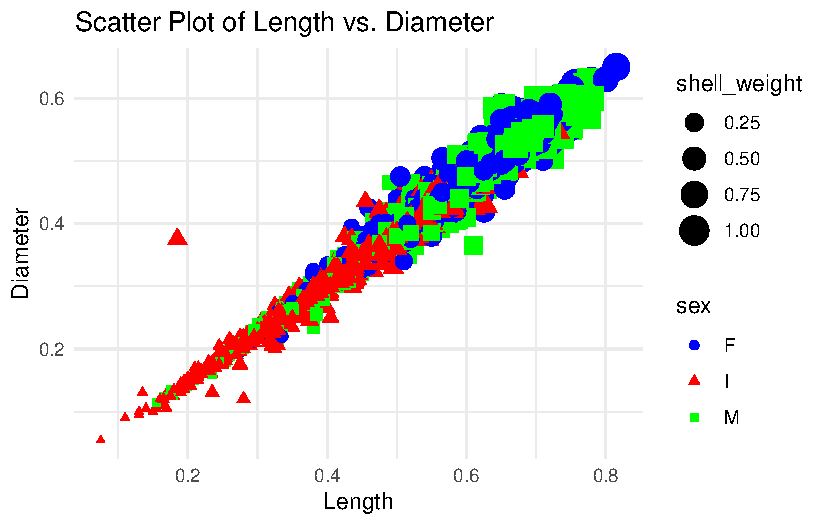
\includegraphics{hw2_files/figure-pdf/unnamed-chunk-7-1.pdf}

}

\end{figure}

\begin{center}\rule{0.5\linewidth}{0.5pt}\end{center}

1.6 (5 points)

For each \texttt{sex}, create separate scatter plots of \texttt{length}
and \texttt{diameter}. For each plot, also add a \textbf{linear}
trendline to illustrate the relationship between the variables. Use the
\texttt{facet\_wrap()} function in R for this, and ensure that the plots
are vertically stacked \textbf{not} horizontally. You should end up with
a plot that looks like this: \footnote{Plot example for 1.6}

\begin{Shaded}
\begin{Highlighting}[]
\FunctionTok{ggplot}\NormalTok{(abalone, }\FunctionTok{aes}\NormalTok{(}\AttributeTok{x =}\NormalTok{ length, }\AttributeTok{y =}\NormalTok{ diameter, }\AttributeTok{color =}\NormalTok{ sex)) }\SpecialCharTok{+}
  \FunctionTok{geom\_point}\NormalTok{() }\SpecialCharTok{+}
  \FunctionTok{geom\_smooth}\NormalTok{(}\AttributeTok{method =} \StringTok{"lm"}\NormalTok{, }\AttributeTok{se =} \ConstantTok{FALSE}\NormalTok{) }\SpecialCharTok{+}
  \FunctionTok{labs}\NormalTok{(}\AttributeTok{title =} \StringTok{"Scatter Plot of Length vs. Diameter by Sex"}\NormalTok{,}
       \AttributeTok{x =} \StringTok{"Length"}\NormalTok{, }\AttributeTok{y =} \StringTok{"Diameter"}\NormalTok{) }\SpecialCharTok{+}
  \FunctionTok{facet\_wrap}\NormalTok{(}\SpecialCharTok{\textasciitilde{}}\NormalTok{ sex, }\AttributeTok{nrow =} \DecValTok{2}\NormalTok{) }\SpecialCharTok{+}
  \FunctionTok{theme\_minimal}\NormalTok{()}
\end{Highlighting}
\end{Shaded}

\begin{verbatim}
`geom_smooth()` using formula = 'y ~ x'
\end{verbatim}

\begin{figure}[H]

{\centering 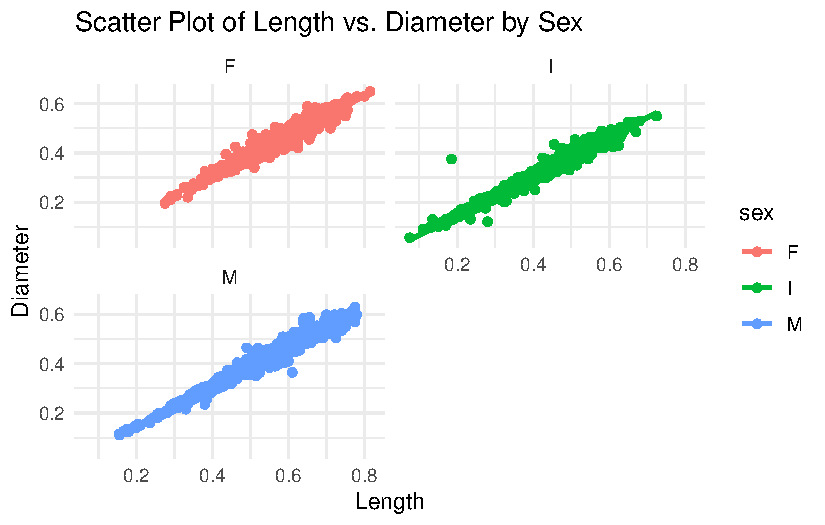
\includegraphics{hw2_files/figure-pdf/unnamed-chunk-8-1.pdf}

}

\end{figure}

---

\hypertarget{question-2}{%
\subsection{Question 2}\label{question-2}}

\begin{tcolorbox}[enhanced jigsaw, opacityback=0, colback=white, rightrule=.15mm, colframe=quarto-callout-tip-color-frame, opacitybacktitle=0.6, title=\textcolor{quarto-callout-tip-color}{\faLightbulb}\hspace{0.5em}{40 points}, breakable, bottomtitle=1mm, arc=.35mm, titlerule=0mm, toptitle=1mm, leftrule=.75mm, left=2mm, bottomrule=.15mm, toprule=.15mm, coltitle=black, colbacktitle=quarto-callout-tip-color!10!white]

More advanced analyses using \texttt{dplyr}, \texttt{purrrr} and
\texttt{ggplot2}

\end{tcolorbox}

\begin{center}\rule{0.5\linewidth}{0.5pt}\end{center}

2.1 (10 points)

Filter the data to only include abalone with a length of at least
\(0.5\) meters. Group the data by \texttt{sex} and calculate the mean of
each variable for each group. Create a bar plot to visualize the mean
values for each variable by \texttt{sex}.

\begin{Shaded}
\begin{Highlighting}[]
\NormalTok{high\_length\_abalone }\OtherTok{\textless{}{-}}\NormalTok{ abalone }\SpecialCharTok{\%\textgreater{}\%}
  \FunctionTok{group\_by}\NormalTok{(sex) }\SpecialCharTok{\%\textgreater{}\%}
  \FunctionTok{filter}\NormalTok{(length }\SpecialCharTok{\textgreater{}=} \FloatTok{0.5}\NormalTok{) }\SpecialCharTok{\%\textgreater{}\%}
  \FunctionTok{summarise}\NormalTok{(}\FunctionTok{across}\NormalTok{(}
    \FunctionTok{c}\NormalTok{(length, diameter, height, whole\_weight, shucked\_weight, viscera\_weight, shell\_weight, rings),}
\NormalTok{    mean,}
    \AttributeTok{na.rm =} \ConstantTok{TRUE}
\NormalTok{  ))}
\end{Highlighting}
\end{Shaded}

\begin{verbatim}
Warning: There was 1 warning in `summarise()`.
i In argument: `across(...)`.
i In group 1: `sex = "F"`.
Caused by warning:
! The `...` argument of `across()` is deprecated as of dplyr 1.1.0.
Supply arguments directly to `.fns` through an anonymous function instead.

  # Previously
  across(a:b, mean, na.rm = TRUE)

  # Now
  across(a:b, \(x) mean(x, na.rm = TRUE))
\end{verbatim}

\begin{Shaded}
\begin{Highlighting}[]
\NormalTok{high\_length\_longer }\OtherTok{\textless{}{-}}\NormalTok{ high\_length\_abalone }\SpecialCharTok{\%\textgreater{}\%}
  \FunctionTok{pivot\_longer}\NormalTok{(}
    \AttributeTok{cols =} \SpecialCharTok{!}\NormalTok{sex,}
    \AttributeTok{names\_to =} \StringTok{"Attributes"}\NormalTok{,}
    \AttributeTok{values\_to =} \StringTok{"Values"}
\NormalTok{  )}

\FunctionTok{ggplot}\NormalTok{(}\AttributeTok{data =}\NormalTok{ high\_length\_longer, }\FunctionTok{aes}\NormalTok{(}\AttributeTok{x =}\NormalTok{ Attributes, }\AttributeTok{y =}\NormalTok{ Values)) }\SpecialCharTok{+}
  \FunctionTok{geom\_col}\NormalTok{() }\SpecialCharTok{+}  
  \FunctionTok{facet\_wrap}\NormalTok{(}\SpecialCharTok{\textasciitilde{}}\NormalTok{sex, }\AttributeTok{ncol =} \DecValTok{1}\NormalTok{) }\SpecialCharTok{+} 
  \FunctionTok{labs}\NormalTok{(}
    \AttributeTok{title =} \StringTok{"Mean Measurements of High{-}Length Abalone"}\NormalTok{,}
    \AttributeTok{x =} \StringTok{"Attributes"}\NormalTok{,}
    \AttributeTok{y =} \StringTok{"Mean Values"}
\NormalTok{  )}
\end{Highlighting}
\end{Shaded}

\begin{figure}[H]

{\centering 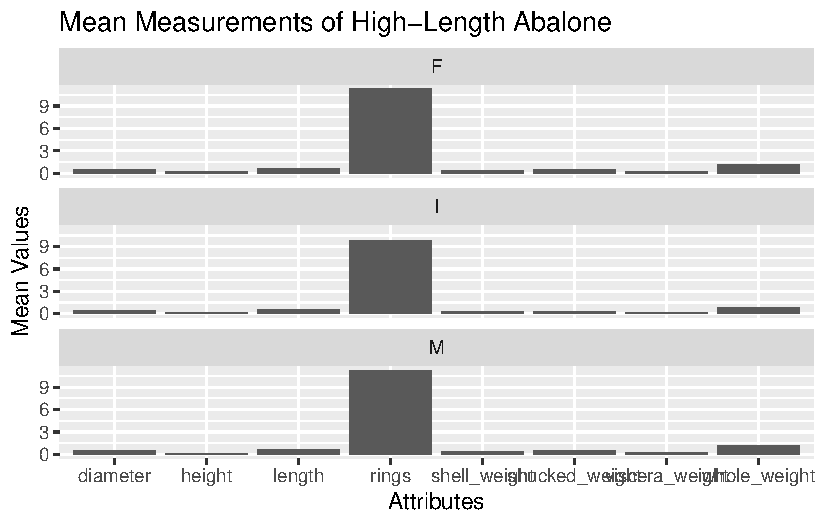
\includegraphics{hw2_files/figure-pdf/unnamed-chunk-9-1.pdf}

}

\end{figure}

\begin{center}\rule{0.5\linewidth}{0.5pt}\end{center}

2.2 (15 points)

Implement the following in a \textbf{single command}:

\begin{enumerate}
\def\labelenumi{\arabic{enumi}.}
\tightlist
\item
  Temporarily create a new variable called \texttt{num\_rings} which
  takes a value of:
\end{enumerate}

\begin{itemize}
\tightlist
\item
  \texttt{"low"} if \texttt{rings\ \textless{}\ 10}
\item
  \texttt{"high"} if \texttt{rings\ \textgreater{}\ 20}, and
\item
  \texttt{"med"} otherwise
\end{itemize}

\begin{enumerate}
\def\labelenumi{\arabic{enumi}.}
\setcounter{enumi}{1}
\item
  Group \texttt{df} by this new variable and \texttt{sex} and compute
  \texttt{avg\_weight} as the average of the
  \texttt{whole\_weight\ +\ shucked\_weight\ +\ viscera\_weight\ +\ shell\_weight}
  for each combination of \texttt{num\_rings} and \texttt{sex}.
\item
  Use the \texttt{geom\_tile()} function to create a tile plot of
  \texttt{num\_rings} vs \texttt{sex} with the color indicating of each
  tile indicating the \texttt{avg\_weight} value.
\end{enumerate}

\begin{Shaded}
\begin{Highlighting}[]
\NormalTok{abalone }\SpecialCharTok{\%\textgreater{}\%}
  \FunctionTok{mutate}\NormalTok{(}\AttributeTok{num\_rings =} \FunctionTok{case\_when}\NormalTok{(}
\NormalTok{    rings }\SpecialCharTok{\textless{}} \DecValTok{10} \SpecialCharTok{\textasciitilde{}} \StringTok{"low"}\NormalTok{,}
\NormalTok{    rings }\SpecialCharTok{\textgreater{}} \DecValTok{20} \SpecialCharTok{\textasciitilde{}} \StringTok{"high"}\NormalTok{,}
    \ConstantTok{TRUE} \SpecialCharTok{\textasciitilde{}} \StringTok{"med"}
\NormalTok{  )) }\SpecialCharTok{\%\textgreater{}\%}
  \FunctionTok{group\_by}\NormalTok{(num\_rings, sex) }\SpecialCharTok{\%\textgreater{}\%}
  \FunctionTok{summarise}\NormalTok{(}\AttributeTok{avg\_weight =} \FunctionTok{mean}\NormalTok{(whole\_weight }\SpecialCharTok{+}\NormalTok{ shucked\_weight }\SpecialCharTok{+}\NormalTok{ viscera\_weight }\SpecialCharTok{+}\NormalTok{ shell\_weight, }\AttributeTok{na.rm =} \ConstantTok{TRUE}\NormalTok{)) }\SpecialCharTok{\%\textgreater{}\%}
  \FunctionTok{ggplot}\NormalTok{(}\FunctionTok{aes}\NormalTok{(}\AttributeTok{x =}\NormalTok{ sex, }\AttributeTok{y =}\NormalTok{ num\_rings, }\AttributeTok{fill =}\NormalTok{ avg\_weight)) }\SpecialCharTok{+}
  \FunctionTok{geom\_tile}\NormalTok{(}\AttributeTok{color =} \StringTok{"white"}\NormalTok{) }\SpecialCharTok{+}
  \FunctionTok{scale\_fill\_gradient}\NormalTok{(}\AttributeTok{low =} \StringTok{"lightblue"}\NormalTok{, }\AttributeTok{high =} \StringTok{"darkblue"}\NormalTok{) }\SpecialCharTok{+}
  \FunctionTok{labs}\NormalTok{(}
    \AttributeTok{title =} \StringTok{"Average Weight by Rings and Sex"}\NormalTok{,}
    \AttributeTok{x =} \StringTok{"Sex"}\NormalTok{,}
    \AttributeTok{y =} \StringTok{"Number of Rings"}\NormalTok{,}
    \AttributeTok{fill =} \StringTok{"Average Weight"}
\NormalTok{  )}
\end{Highlighting}
\end{Shaded}

\begin{verbatim}
`summarise()` has grouped output by 'num_rings'. You can override using the
`.groups` argument.
\end{verbatim}

\begin{figure}[H]

{\centering 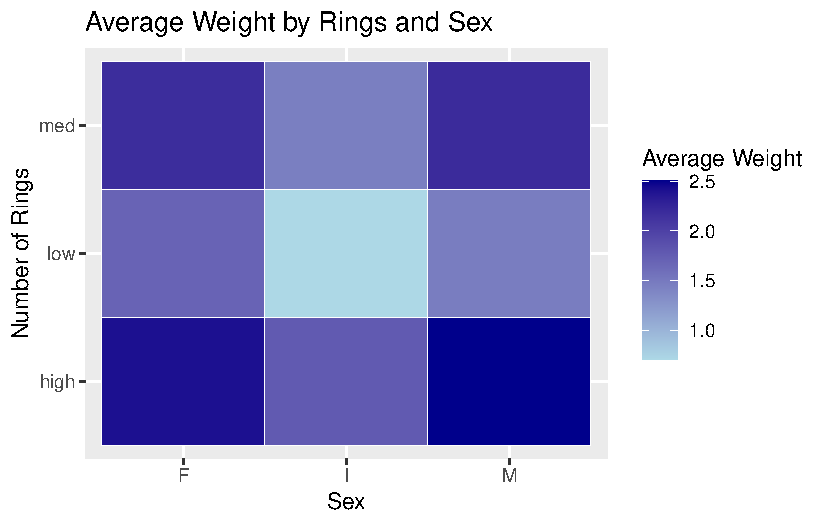
\includegraphics{hw2_files/figure-pdf/unnamed-chunk-10-1.pdf}

}

\end{figure}

\begin{center}\rule{0.5\linewidth}{0.5pt}\end{center}

2.3 (5 points)

Make a table of the pairwise correlations between all the numeric
variables rounded to 2 decimal points. Your final answer should look
like this \footnote{Table for 2.3}

\begin{Shaded}
\begin{Highlighting}[]
\NormalTok{numeric\_vars }\OtherTok{\textless{}{-}} \FunctionTok{select\_if}\NormalTok{(df, is.numeric)}

\NormalTok{correlation\_matrix }\OtherTok{\textless{}{-}} \FunctionTok{round}\NormalTok{(}\FunctionTok{cor}\NormalTok{(numeric\_vars), }\DecValTok{2}\NormalTok{)}

\FunctionTok{print}\NormalTok{(correlation\_matrix)}
\end{Highlighting}
\end{Shaded}

\begin{verbatim}
               length diameter height whole_weight shucked_weight
length           1.00     0.99   0.83         0.93           0.90
diameter         0.99     1.00   0.83         0.93           0.89
height           0.83     0.83   1.00         0.82           0.77
whole_weight     0.93     0.93   0.82         1.00           0.97
shucked_weight   0.90     0.89   0.77         0.97           1.00
viscera_weight   0.90     0.90   0.80         0.97           0.93
shell_weight     0.90     0.91   0.82         0.96           0.88
rings            0.56     0.57   0.56         0.54           0.42
               viscera_weight shell_weight rings
length                   0.90         0.90  0.56
diameter                 0.90         0.91  0.57
height                   0.80         0.82  0.56
whole_weight             0.97         0.96  0.54
shucked_weight           0.93         0.88  0.42
viscera_weight           1.00         0.91  0.50
shell_weight             0.91         1.00  0.63
rings                    0.50         0.63  1.00
\end{verbatim}

\begin{center}\rule{0.5\linewidth}{0.5pt}\end{center}

2.4 (10 points)

Use the \texttt{map2()} function from the \texttt{purrr} package to
create a scatter plot for each \emph{quantitative} variable against the
number of \texttt{rings} variable. Color the points based on the
\texttt{sex} of each abalone. You can use the
\texttt{cowplot::plot\_grid()} function to finally make the following
grid of plots.

\begin{Shaded}
\begin{Highlighting}[]
\NormalTok{quantitative\_vars }\OtherTok{\textless{}{-}} \FunctionTok{select}\NormalTok{(abalone, }\SpecialCharTok{{-}}\NormalTok{sex) }\SpecialCharTok{\%\textgreater{}\%}
  \FunctionTok{keep}\NormalTok{(is.numeric)}

\NormalTok{scatter\_plots }\OtherTok{\textless{}{-}} \FunctionTok{map2}\NormalTok{(quantitative\_vars, }\FunctionTok{names}\NormalTok{(quantitative\_vars), }\SpecialCharTok{\textasciitilde{}}
                        \FunctionTok{ggplot}\NormalTok{(abalone, }\FunctionTok{aes}\NormalTok{(}\AttributeTok{x =}\NormalTok{ .data[[.y]], }\AttributeTok{y =}\NormalTok{ rings, }\AttributeTok{color =}\NormalTok{ sex)) }\SpecialCharTok{+}
                          \FunctionTok{geom\_point}\NormalTok{() }\SpecialCharTok{+}
                          \FunctionTok{labs}\NormalTok{(}\AttributeTok{x =}\NormalTok{ .y, }\AttributeTok{y =} \StringTok{"Number of Rings"}\NormalTok{) }\SpecialCharTok{+}
                          \FunctionTok{theme\_minimal}\NormalTok{())}

\FunctionTok{plot\_grid}\NormalTok{(}\AttributeTok{plotlist =}\NormalTok{ scatter\_plots, }\AttributeTok{ncol =} \DecValTok{2}\NormalTok{)}
\end{Highlighting}
\end{Shaded}

\begin{figure}[H]

{\centering 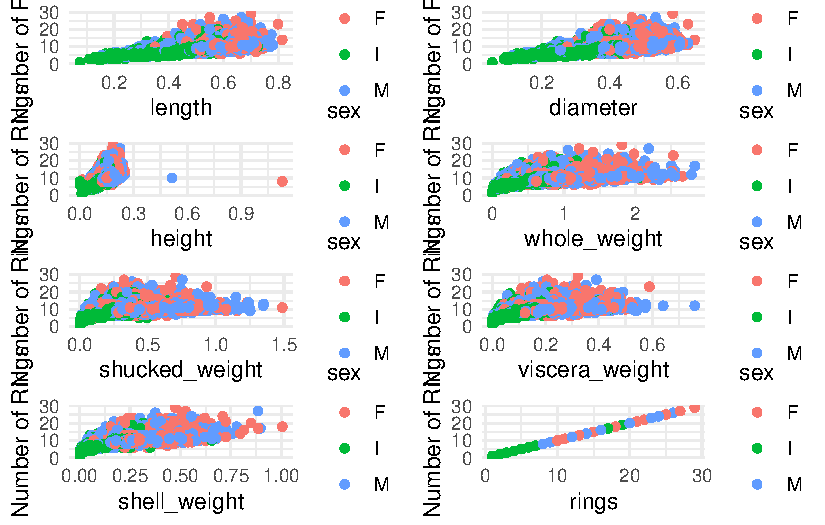
\includegraphics{hw2_files/figure-pdf/unnamed-chunk-12-1.pdf}

}

\end{figure}

---

\hypertarget{question-3}{%
\subsection{Question 3}\label{question-3}}

\begin{tcolorbox}[enhanced jigsaw, opacityback=0, colback=white, rightrule=.15mm, colframe=quarto-callout-tip-color-frame, opacitybacktitle=0.6, title=\textcolor{quarto-callout-tip-color}{\faLightbulb}\hspace{0.5em}{30 points}, breakable, bottomtitle=1mm, arc=.35mm, titlerule=0mm, toptitle=1mm, leftrule=.75mm, left=2mm, bottomrule=.15mm, toprule=.15mm, coltitle=black, colbacktitle=quarto-callout-tip-color!10!white]

Linear regression using \texttt{lm}

\end{tcolorbox}

\begin{center}\rule{0.5\linewidth}{0.5pt}\end{center}

3.1 (10 points)

Perform a simple linear regression with \texttt{diameter} as the
covariate and \texttt{height} as the response. Interpret the model
coefficients and their significance values.

\begin{Shaded}
\begin{Highlighting}[]
\NormalTok{model }\OtherTok{\textless{}{-}} \FunctionTok{lm}\NormalTok{(height }\SpecialCharTok{\textasciitilde{}}\NormalTok{ diameter, }\AttributeTok{data =}\NormalTok{ abalone)}

\FunctionTok{summary}\NormalTok{(model)}
\end{Highlighting}
\end{Shaded}

\begin{verbatim}

Call:
lm(formula = height ~ diameter, data = abalone)

Residuals:
     Min       1Q   Median       3Q      Max 
-0.15513 -0.01053 -0.00147  0.00852  1.00906 

Coefficients:
             Estimate Std. Error t value Pr(>|t|)    
(Intercept) -0.003803   0.001512  -2.515   0.0119 *  
diameter     0.351376   0.003602  97.544   <2e-16 ***
---
Signif. codes:  0 '***' 0.001 '**' 0.01 '*' 0.05 '.' 0.1 ' ' 1

Residual standard error: 0.0231 on 4175 degrees of freedom
Multiple R-squared:  0.695, Adjusted R-squared:  0.695 
F-statistic:  9515 on 1 and 4175 DF,  p-value: < 2.2e-16
\end{verbatim}

\begin{center}\rule{0.5\linewidth}{0.5pt}\end{center}

3.2 (10 points)

Make a scatterplot of \texttt{height} vs \texttt{diameter} and plot the
regression line in \texttt{color="red"}. You can use the base
\texttt{plot()} function in R for this. Is the linear model an
appropriate fit for this relationship? Explain.

\begin{Shaded}
\begin{Highlighting}[]
\FunctionTok{plot}\NormalTok{(abalone}\SpecialCharTok{$}\NormalTok{diameter, df}\SpecialCharTok{$}\NormalTok{height, }\AttributeTok{xlab =} \StringTok{"Diameter"}\NormalTok{, }\AttributeTok{ylab =} \StringTok{"Height"}\NormalTok{, }\AttributeTok{main =} \StringTok{"Scatterplot of Height vs Diameter"}\NormalTok{)}

\NormalTok{model }\OtherTok{\textless{}{-}} \FunctionTok{lm}\NormalTok{(height }\SpecialCharTok{\textasciitilde{}}\NormalTok{ diameter, }\AttributeTok{data =}\NormalTok{ abalone)}

\FunctionTok{abline}\NormalTok{(model, }\AttributeTok{col =} \StringTok{"red"}\NormalTok{)}
\end{Highlighting}
\end{Shaded}

\begin{figure}[H]

{\centering 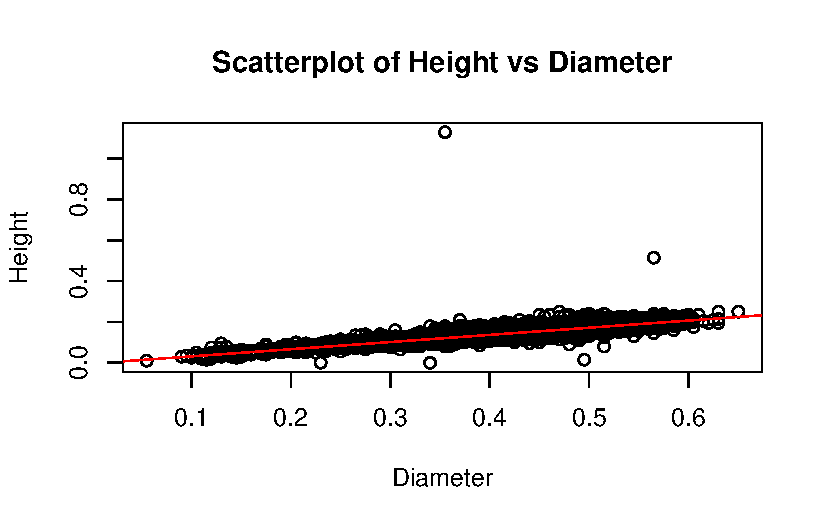
\includegraphics{hw2_files/figure-pdf/unnamed-chunk-14-1.pdf}

}

\end{figure}

\begin{center}\rule{0.5\linewidth}{0.5pt}\end{center}

3.3 (10 points)

Suppose we have collected observations for ``new'' abalones with
\texttt{new\_diameter} values given below. What is the expected value of
their \texttt{height} based on your model above? Plot these new
observations along with your predictions in your plot from earlier using
\texttt{color="violet"}

\begin{Shaded}
\begin{Highlighting}[]
\NormalTok{  new\_diameters }\OtherTok{\textless{}{-}} \FunctionTok{c}\NormalTok{(}
    \FloatTok{0.15218946}\NormalTok{,}
    \FloatTok{0.48361548}\NormalTok{,}
    \FloatTok{0.58095513}\NormalTok{,}
    \FloatTok{0.07603687}\NormalTok{,}
    \FloatTok{0.50234599}\NormalTok{,}
    \FloatTok{0.83462092}\NormalTok{,}
    \FloatTok{0.95681938}\NormalTok{,}
    \FloatTok{0.92906875}\NormalTok{,}
    \FloatTok{0.94245437}\NormalTok{,}
    \FloatTok{0.01209518}
\NormalTok{  )}
  
\NormalTok{new\_data }\OtherTok{\textless{}{-}} \FunctionTok{data.frame}\NormalTok{(}\AttributeTok{diameter =}\NormalTok{ new\_diameters)}

\NormalTok{new\_data}\SpecialCharTok{$}\NormalTok{predicted\_height }\OtherTok{\textless{}{-}} \FunctionTok{predict}\NormalTok{(model, }\AttributeTok{newdata =}\NormalTok{ new\_data)}

\FunctionTok{plot}\NormalTok{(abalone}\SpecialCharTok{$}\NormalTok{diameter, abalone}\SpecialCharTok{$}\NormalTok{height, }\AttributeTok{xlab =} \StringTok{"Diameter"}\NormalTok{, }\AttributeTok{ylab =} \StringTok{"Height"}\NormalTok{, }\AttributeTok{main =} \StringTok{"Scatterplot of Height vs Diameter"}\NormalTok{, }\AttributeTok{col =} \StringTok{"black"}\NormalTok{)}
\FunctionTok{abline}\NormalTok{(model, }\AttributeTok{col =} \StringTok{"red"}\NormalTok{)}

\FunctionTok{points}\NormalTok{(new\_data}\SpecialCharTok{$}\NormalTok{diameter, new\_data}\SpecialCharTok{$}\NormalTok{predicted\_height, }\AttributeTok{col =} \StringTok{"violet"}\NormalTok{, }\AttributeTok{pch =} \DecValTok{19}\NormalTok{)}
\FunctionTok{legend}\NormalTok{(}\StringTok{"topleft"}\NormalTok{, }\AttributeTok{legend =} \StringTok{"Predictions"}\NormalTok{, }\AttributeTok{pch =} \DecValTok{19}\NormalTok{, }\AttributeTok{col =} \StringTok{"violet"}\NormalTok{, }\AttributeTok{bty =} \StringTok{"n"}\NormalTok{)}
\end{Highlighting}
\end{Shaded}

\begin{figure}[H]

{\centering 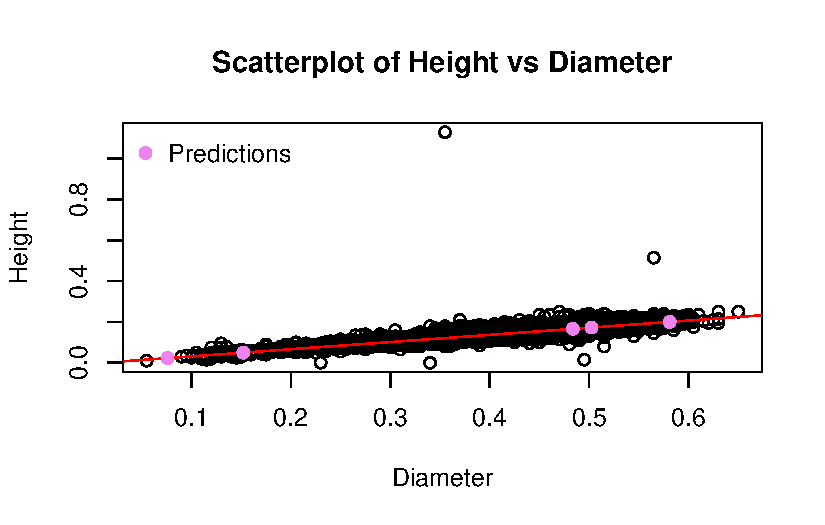
\includegraphics{hw2_files/figure-pdf/unnamed-chunk-15-1.pdf}

}

\end{figure}

\pagebreak

---

\hypertarget{appendix}{%
\section{Appendix}\label{appendix}}

\begin{tcolorbox}[enhanced jigsaw, opacityback=0, colback=white, rightrule=.15mm, colframe=quarto-callout-note-color-frame, opacitybacktitle=0.6, title=\textcolor{quarto-callout-note-color}{\faInfo}\hspace{0.5em}{Session Information}, breakable, bottomtitle=1mm, arc=.35mm, titlerule=0mm, toptitle=1mm, leftrule=.75mm, left=2mm, bottomrule=.15mm, toprule=.15mm, coltitle=black, colbacktitle=quarto-callout-note-color!10!white]

Print your \texttt{R} session information using the following command

\begin{Shaded}
\begin{Highlighting}[]
\FunctionTok{sessionInfo}\NormalTok{()}
\end{Highlighting}
\end{Shaded}

\begin{verbatim}
R version 4.3.2 (2023-10-31 ucrt)
Platform: x86_64-w64-mingw32/x64 (64-bit)
Running under: Windows 11 x64 (build 22621)

Matrix products: default


locale:
[1] LC_COLLATE=English_United States.utf8 
[2] LC_CTYPE=English_United States.utf8   
[3] LC_MONETARY=English_United States.utf8
[4] LC_NUMERIC=C                          
[5] LC_TIME=English_United States.utf8    

time zone: America/New_York
tzcode source: internal

attached base packages:
[1] stats     graphics  grDevices datasets  utils     methods   base     

other attached packages:
[1] cowplot_1.1.3 purrr_1.0.2   dplyr_1.1.4   ggplot2_3.4.4 tidyr_1.3.1  
[6] readr_2.1.5  

loaded via a namespace (and not attached):
 [1] Matrix_1.6-1.1   bit_4.0.5        gtable_0.3.4     jsonlite_1.8.8  
 [5] crayon_1.5.2     compiler_4.3.2   renv_1.0.3       tidyselect_1.2.0
 [9] parallel_4.3.2   splines_4.3.2    scales_1.3.0     yaml_2.3.8      
[13] fastmap_1.1.1    lattice_0.21-9   R6_2.5.1         labeling_0.4.3  
[17] generics_0.1.3   curl_5.2.0       knitr_1.45       tibble_3.2.1    
[21] munsell_0.5.0    pillar_1.9.0     tzdb_0.4.0       rlang_1.1.3     
[25] utf8_1.2.4       xfun_0.42        bit64_4.0.5      cli_3.6.2       
[29] mgcv_1.9-0       withr_3.0.0      magrittr_2.0.3   digest_0.6.34   
[33] grid_4.3.2       vroom_1.6.5      hms_1.1.3        nlme_3.1-163    
[37] lifecycle_1.0.4  vctrs_0.6.5      evaluate_0.23    glue_1.7.0      
[41] farver_2.1.1     fansi_1.0.6      colorspace_2.1-0 rmarkdown_2.25  
[45] tools_4.3.2      pkgconfig_2.0.3  htmltools_0.5.7 
\end{verbatim}

\end{tcolorbox}

::: \{.content-visible when-format=``html''\} \textbar{} length
\textbar{} diameter \textbar{} height \textbar{} whole\_weight
\textbar{} shucked\_weight \textbar{} viscera\_weight \textbar{}
shell\_weight \textbar{} rings \textbar{} \textbar{}
\textbar:-------\textbar-------:\textbar-------:\textbar-------:\textbar-------:\textbar-------:\textbar-------:\textbar-------:\textbar-------:\textbar{}
\textbar{} length \textbar{} 1.00 \textbar{} 0.99 \textbar{} 0.83
\textbar{} 0.93 \textbar{} 0.90 \textbar{} 0.90 \textbar{} 0.90
\textbar{} 0.56 \textbar{} \textbar{} diameter \textbar{} 0.99
\textbar{} 1.00 \textbar{} 0.83 \textbar{} 0.93 \textbar{} 0.89
\textbar{} 0.90 \textbar{} 0.91 \textbar{} 0.57 \textbar{} \textbar{}
height \textbar{} 0.83 \textbar{} 0.83 \textbar{} 1.00 \textbar{} 0.82
\textbar{} 0.77 \textbar{} 0.80 \textbar{} 0.82 \textbar{} 0.56
\textbar{} \textbar{} whole\_weight \textbar{} 0.93 \textbar{} 0.93
\textbar{} 0.82 \textbar{} 1.00 \textbar{} 0.97 \textbar{} 0.97
\textbar{} 0.96 \textbar{} 0.54 \textbar{} \textbar{} shucked\_weight
\textbar{} 0.90 \textbar{} 0.89 \textbar{} 0.77 \textbar{} 0.97
\textbar{} 1.00 \textbar{} 0.93 \textbar{} 0.88 \textbar{} 0.42
\textbar{} \textbar{} viscera\_weight \textbar{} 0.90 \textbar{} 0.90
\textbar{} 0.80 \textbar{} 0.97 \textbar{} 0.93 \textbar{} 1.00
\textbar{} 0.91 \textbar{} 0.50 \textbar{} \textbar{} shell\_weight
\textbar{} 0.90 \textbar{} 0.91 \textbar{} 0.82 \textbar{} 0.96
\textbar{} 0.88 \textbar{} 0.91 \textbar{} 1.00 \textbar{} 0.63
\textbar{} \textbar{} rings \textbar{} 0.56 \textbar{} 0.57 \textbar{}
0.56 \textbar{} 0.54 \textbar{} 0.42 \textbar{} 0.50 \textbar{} 0.63
\textbar{} 1.00 \textbar{}



\end{document}
